\section{Motivation} \label{sec:motiv}

\subsection{Insights}

\begin{figure}
  \begin{center}
    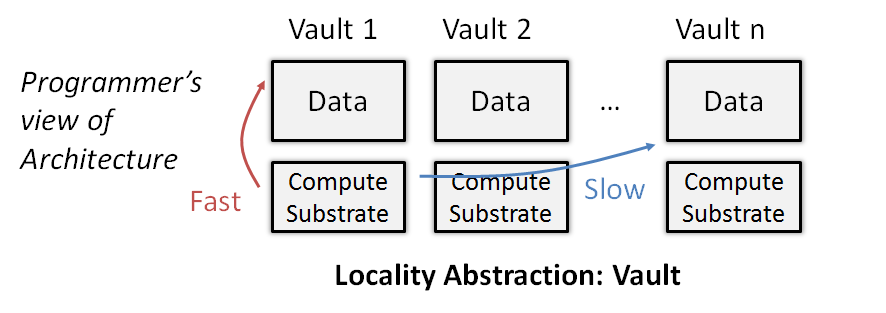
\includegraphics[width=\linewidth]{cs758-figs/prog-abs.png}
  \end{center}
\vspace{-0.2in}
  \caption{Programmer Abstraction of the Architecture}
  \label{fig:prog-overview}
\vspace{-0.05in}
\end{figure}


\subsection{Mechanisms to Exploit Inisghts}

\paragraph{Programmer View of Architecture}
We first describe the programmer view of the proximate archietcture, 
based on the insights and mechanisms discussed ealrier in Section~\ref{sec:motiv} 
The high level question one has to ask in how to give the programmers control
of data and task locality within proximate cores?. We answer this
in Porximate by providing a flexible programming model to enable the 
programmer managed data sharding and task/data co-location. 
Figure~\ref{fig:prog-overview} shows the programmers's view of the archietcture, 
and the vault abstraction proximate provides. Each vault is group of cores
and a predetermined slice of virutal address spaces, exposed during task offloading 
and memory allocation. 

The locality abstraction for programmers is given by the vault. Each vault, 
has an address parition (data) and the compute substrate to work or offload task
on that address parition. 


